\documentclass[11pt, a4paper]{article}
\usepackage{minted}
\usepackage{multirow}
\usepackage{enumerate}
\usepackage{geometry}
\usepackage{array}
\geometry{left=2.5cm,right=2.5cm,top=2.5cm,bottom=2.5cm}
%\usepackage{minted}
\usepackage[slantfont,boldfont]{xeCJK}
\setCJKmainfont{SimSun}
\usepackage{indentfirst}
\usepackage{float}
\setlength{\parindent}{2em}
\setCJKmonofont{SimHei}
\input zhwinfonts
\renewcommand\figurename{图}
\renewcommand\tablename{表}
\renewcommand\contentsname{\centering 目录}

\begin{document}

\begin{center}
  {\bf \Huge 2017年春季学期本科生课程考核}
\end{center}

\title{{\bf 对一种位图索引UpBit\cite{art1}的研究}\\软件设计与开发实践I课程报告}
\renewcommand\arraystretch{2}
\begin{table}[H]
\centering
\begin{tabular}{|p{3cm}<{\centering}|p{3cm}<{\centering}|p{3cm}<{\centering}|p{3cm}<{\centering}|}
  \hline
考核科目     & \multicolumn{3}{c|}{软件设计与开发实践I} \\ \hline
学生所在院(系) & \multicolumn{3}{c|}{计算机学院}      \\ \hline
学生所在学科   & \multicolumn{3}{c|}{计算机科学与技术}   \\ \hline
学生姓名     & \multicolumn{3}{c|}{马玉坤}        \\ \hline
学号       & \multicolumn{3}{c|}{1150310618} \\ \hline
考核结果     &          & 阅卷人        &         \\ \hline
\end{tabular}
\end{table}
  \author{计算机科学与技术学院\\马玉坤\\1150310618}
  \date{2017年6月22日}

  \maketitle

  \emph{伴随着科技经济发展与互联网的普及,时代对数据的获取、分析提出了更高的要求。在海量数据领域,数据仓库的地位变得越来越重要。在众多数据仓库的实现方案中,位图索引与B树及其变种被广泛应用。本文从UpBit这种位图索引出发,讨论了位图索引领域部分极为重要的问题,对前人的工作进行举例和比较,并提出了一种对UpBit的改进方法。}\\
  {\bf 关键字:}位图索引,数据仓库,位图压缩,位图编码

  \tableofcontents

  \clearpage

  \section{背景知识}

  \subsection{位图索引}
  位图索引(Bitmap Index)由P’ONeil在1987年提出,并在一个商用数据库系统Model 204上首次应用。在数据库中,无论是用于科研用途,还是商业用途,位图向量都被广泛应用。\cite{art3}最原始的位图索引利用位向量(Bit Vector)来表示某种被索引的属性在数据集中的索引情况。例如在表\ref{tb:table}中:在“数学成绩”一列中“优秀”这个属性的位图向量为101,分别代表小A拥有此属性、小B未拥有此属性,小C拥有此属性。将不同属性的位向量进行位逻辑运算,即可以回答各种复杂的信息。

  \begin{table}[H]
    \centering
    \label{tb:table} \caption{一个普通的表}
    \begin{tabular}{|l|l|l|}
      \hline
      姓名 & 数学成绩 & 语文成绩 \\ \hline
      小A & 优秀   & 及格   \\ \hline
      小B & 良好   & 优秀   \\ \hline
      小C & 优秀   & 不及格 \\ \hline
    \end{tabular}
  \end{table}

  位图索引尽管是被设计来高效地进行大量的数据库查询操作,但相对少量的数据库修改操作有时也是必要的。如何高效地让位图索引在能够进行高效查询的同时进行高效的修改,是数据库领域的热门问题。

  \cite{art1}使用了维护更新向量和分块指针的方法,较好地解决了使用位图向量高效进行查询和修改操作的问题。

  \subsection{对单个位向量的压缩}

  到目前为止,已经有众多有关压缩单个位向量的工作被做出。例如,通用的文字压缩算法,像LZ77,对于减少位向量存储大小十分有效,然而却并不能显著减少查询所需要消耗的时间,因为不同压缩后的位向量进行位操作前必须进行解压缩。对于位向量的压缩方法,通常使用的都是行程长度压缩 ({\bf RLE})方法,即将连续出现的相同的位合并,例如将11110000记做“4个连续的1+4个连续的0”。较为有名的行程长度压缩算法有BBC (Byte-aligned Bitmap Code)和WAH (Word-Alignment Hybrid Code)。

  \subsubsection{BBC (Byte-aligned Bitmap Code)}

  \begin{figure}[H]
    \begin{center}
      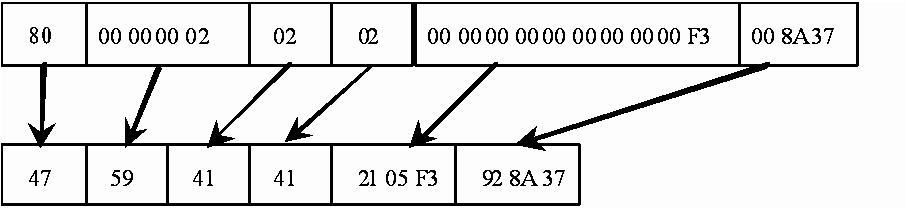
\includegraphics[width=5in]{img/bbc.png}
      \caption{BBC图解}\label{fig:bbc}
    \end{center}
  \end{figure}

  BBC将被压缩的位序列按字节分组为一系列节,压缩后的数据仍然以字节为单位。每节压缩后包括一个 fill 部分和一个 tail 部分。BBC中的字节包括两类:fill 字节和 literal 字节。fill 字节必须为全 1 或全 0,分别称为 1- fill 或 0- fill,literal 字节则按原文 (不压缩) 存放各位。单边 (One- sided) BBC只对 0- fill 压缩,适合于稀疏位图索引,双边 (Two- sided) 。BBC则对 0- fill 和 1- fill 均压缩。一个头字节 (Header byte) 用于表明节的种类。图\ref{fig:bbc}为一个位序列对应的 BBC压缩结果 (所有字节均用十六进制表示) 。

  \subsubsection{WAH (Word-Alignment Hybrid Code)}

  BBC以字节为单位进行位运算,然而计算机的 CPU 以字为单位进行位运算,所以 K. Wu 等人提出了以字为单位的位图索引编码:WAH。为了加快直接在压缩位图上的位运算速度,WAH 采用了更为简单的编码方式。WAH 中没有头字或头字节,这样就消除了压缩数据的前后依赖性,便于 CPU 并行处理。

  \begin{figure}[H]
    \begin{center}
      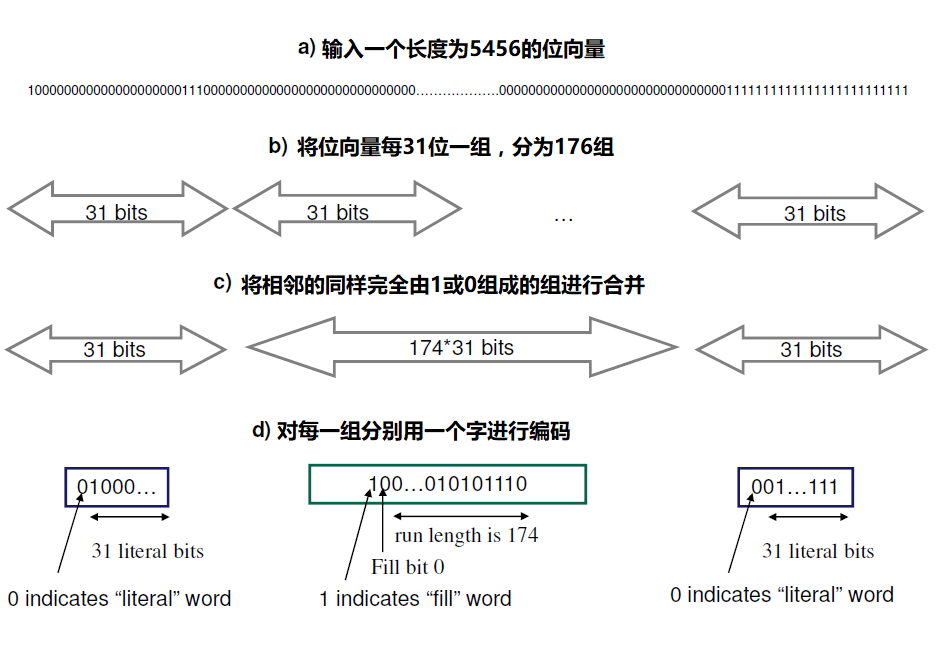
\includegraphics[width=5in]{img/wah.png}
      \caption{WAH图解}\label{fig:wah}
    \end{center}
  \end{figure}

  WAH 中只有两类字:literal 字和 fill 字,用最高位以示区别 (0 为 literal,1为 fill) 。令计算机的字长为 w,则 literal 字可保存 w- 1 个位。fill 字的次高位表示重复位是 0 还是 1,余下的 w-2 位则用于表示一个节的长度 (以字为单位) 。图\ref{fig:wah}表示一个位序列对应的 WAH 压缩结果。


  \section{UpBit思想}

  \subsection{Update Conscious Bitvector}

  在\cite{art1}前,已有一种叫做Update Conscious Bitvector(下简称UCB)的支持修改的位图索引技术被提出。该篇论文提出的Upbit即是在UCB的基础上加以改进的成果。UCB的主要思想如下:


  使用WAH\cite{art5}算法对位向量进行压缩后,压缩后的位向量上原地修改的效率堪忧,但是容易发现,在压缩后位向量的最后面添加一位的速度是极快的。对于可修改的位图向量的优化,一个直接想法是,既然修改操作并不多,原地修改的效率堪忧,为什么不把修改操作转化为禁用(删除)+添加操作?这即是UCB(Update Conscious Bitmaps)的主要思想。

  \begin{figure}[H]
    \begin{center}
      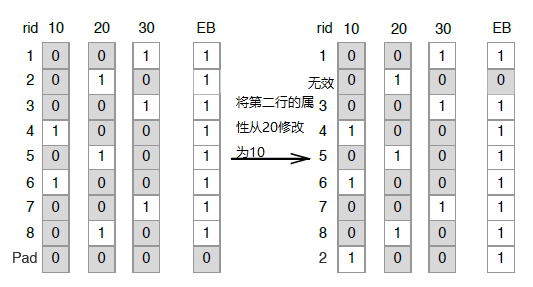
\includegraphics[width=5in]{img/ucb.png}
      \caption{UCB图解} \label{fig:ucb}
    \end{center}
  \end{figure}

  在UCB中,每行都有一个额外的位向量叫做存在向量(Existence Bitvector, EB)。当$EB_i$为1时,表示该行有效,否则该行无效(Invalid)。如图\ref{fig:ucb},当我们想要把第二行的值从20改为10时,我们只需要将$EB_2$设为0,然后在位向量后新建一位,并将对应的EB设为1。

  查询时,我们需要将对应的属性的位向量与存在向量进行“逻辑与”操作。

  实验中,UCB的确能极大地提高伴有少量修改操作的查询效率的提高,但是随着修改操作的积累,存在向量的复杂性将大大提高,UCB查询的效率将会极大地下降。如何使位图向量查询的效率随着修改操作积累不明显提高?这便是Upbit的创新之处。

  \subsection{Upbit}

  实际上,上一个问题的解决方案并不难。既然随着修改次数的增加,EB的复杂度提高,造成了查询的瓶颈。为什么我们不在修改次数达到一定数量级时,通过修改各个属性的位向量来维护存在向量,使存在向量保持高压缩性,提高查询效率?

  UpBit使用了这种策略。UpBit是一个新提出的位图向量方案,能够在保持修改效率较快的情况下,保持查询的效率。

  UpBit并没有只使用一个存在向量,而是对每个属性都使用了一个更新向量(Update Bitvector,UB)。每一个属性的位向量,用两个位向量经“位异或”计算得出,这两个位向量分别为值向量(Value Bitvector,VB)与更新向量(Update Bitvector,UB)。

  由于每一个属性的位向量用两个位向量经“位异或”计算得出。所以无论我们修改UB或者VB,都相当于对属性进行修改。在每次修改操作时,我们直接修改UB的值。如图\ref{fig:upbit},当我们想要把第二行的值从20修改为10,只需要把属性20对应的$UB_i$取反(从0变为1或者从1变为0),然后把属性10对应的$UB_i$取反。

  \begin{figure}[H]
    \begin{center}
      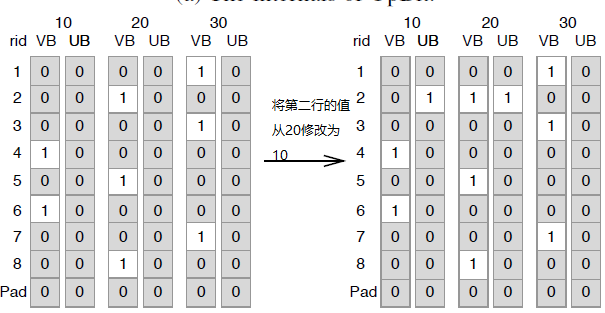
\includegraphics[width=5in]{img/upbit.png}
      \caption{Upbit图解}
      \label{fig:upbit}
    \end{center}
  \end{figure}


  \subsubsection{定时维护更新向量}
  当某个属性的UB的修改次数达到一定阈值时,我们将该属性的VB与UB做异或操作,将结果保存到VB中,然后将UB设为全0的向量,这便是对UB的维护。这样的维护可以保证随着修改操作积累,查询的效率仍然可以很快。

  \subsubsection{维护向量的分块指针}
  同时,UpBit还使用了第二种关键的提高效率的方法——块指针(Fence Pointers)。当我们对某一行的值进行修改时,首先就需要找到这一行修改前的值。在寻找这一行修改前的值的过程中,我们需要在每一个属性的压缩后的UB和VB中查询这一行对应的二进制位的值。如何在压缩后的位向量中,快速找到第i位的值,是一个与效率关系极大的问题。块指针的思想是:将未压缩前的位向量按下标分为若干连续的块,每一块的块大小都接近g(g是人为给定的值)。对于每个位向量,维护每一块的起始位置对应的行在压缩后的位向量中的位置,就可以在O(g+log N/g)的时间复杂度内快速在每个压缩后位向量中找到任意一行的位置,并可在O(N/g)的时间复杂度内维护修改后位向量的块指针。

  \section{基本算法}

  \subsection{获取某一行的值}

  获取第i行的值时,需要枚举值域,直到找到某个值对应的$UB$和$VB$满足$UB_i \oplus VB_i = 1$。

  \begin{figure}[H]
    \begin{center}
      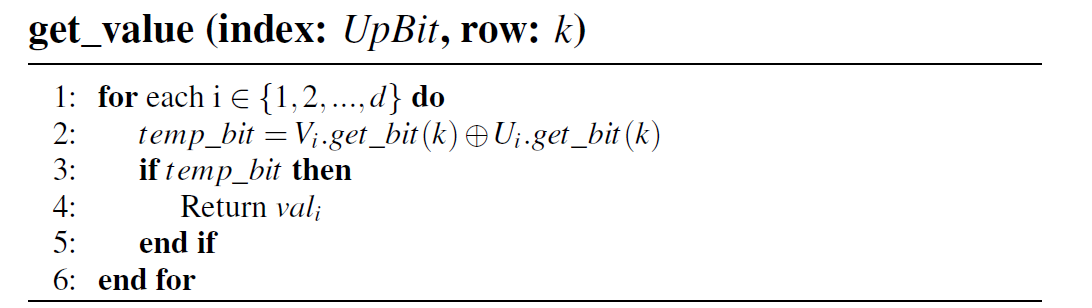
\includegraphics[width=5in]{img/get_value.png}
      \caption{获取某一行的值}
      \label{fig:get_value}
    \end{center}
  \end{figure}

  \subsection{更新某一行的值}

  更新某一行的值时,首先要获取当前行的原始的值(可以使用get\_value()),然后再将两个值对应的$UB_i$都分别进行取反。


  \begin{figure}[H]
    \begin{center}
      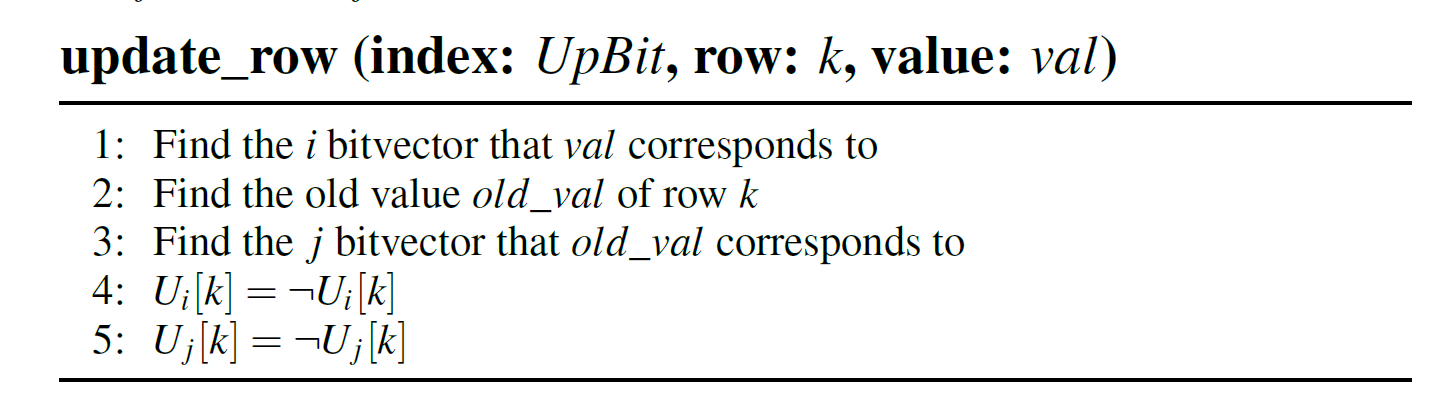
\includegraphics[width=5in]{img/update_row.png}
      \caption{修改某一行的值}
      \label{fig:update_row}
    \end{center}
  \end{figure}

  \subsection{合并UB与VB}

  当UB的修改次数达到一定阈值(阈值需人为设定)时,需要将UB与对应的VB合并,然后将UB置0。下图中FP为Fence Pointers。

  \begin{figure}[H]
    \begin{center}
      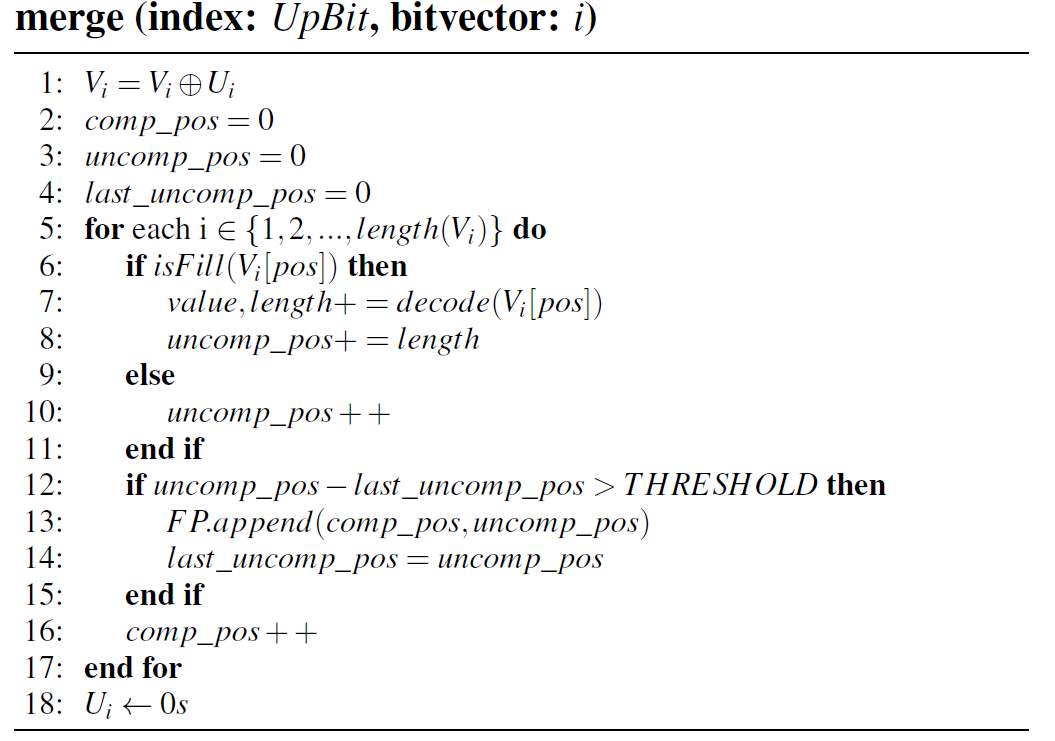
\includegraphics[width=5in]{img/merge.png}
      \caption{合并UB与VB}
      \label{fig:merge}
    \end{center}
  \end{figure}

  \section{算法分析}

  该算法原理巧妙简洁,并能对位图向量的效率带来极大的提升。

  \subsection{空间复杂度分析}

  由于使用了WAH压缩,其空间复杂度为$O(R)$\footnote{设行数为$R$,值域大小为$C$。}。Fence Pointers的空间复杂度与g有关,但仍小于$O(R)$。故总空间复杂度为$O(R)$。

  \subsection{时间复杂度分析}

  查询某一行的值的时间复杂度为$O(C(g + \log \frac{R}{g}))$,修改某一行的值时,由于比查询多了维护Fence Pointers的代价,故时间复杂度为$O(C(g + \log \frac{R}{g} + R/g))$。


\section{对UpBit优化的动机}
\subsection{时间效率}
\subsubsection{对行查询}
\begin{itemize}
\item 更新第k行的值,需要找到第k行修改之前的值。
\item 然而,如图\ref{fig:get_value},寻找第k行的值最坏情况下要遍历所有的位向量。
\item 实际上,作者实验证明,在基数 ({\bf distinct cardinality})等于1000时,get\_value函数耗时占update总耗时的93\%。
\end{itemize}
\begin{figure}[H]
  \begin{center}
    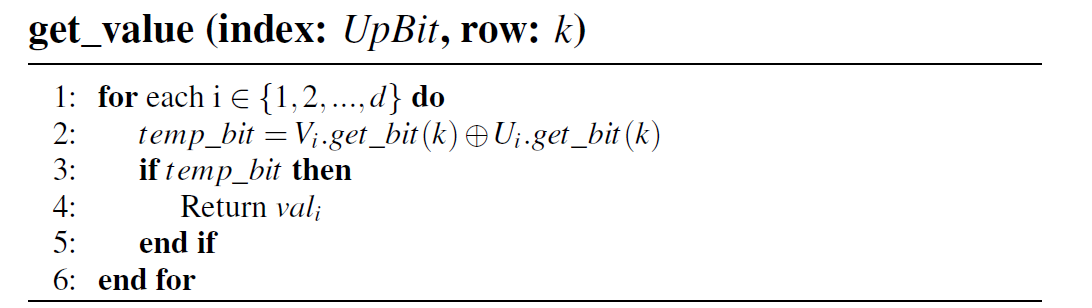
\includegraphics[width=4.8in]{img/get_value.png}
    \caption{UpBit对行查询}\label{fig:get_value}
  \end{center}
\end{figure}

\subsubsection{范围查询}
  在对数据库查询(例如使用SQL语句)时,我们经常会用到范围查询,比如\\\mintinline{sql}{SELECT * FROM Persons WHERE Year>1965}。

  然而,直接使用UpBit进行范围查询的效率是较低的。最坏情况下需要遍历所有的位向量。

\subsection{空间效率}
\subsubsection{对Update BitVectors的正确认识}
实际上,Update BitVectors在UpBit中起了缓存的作用。而在计算机中,缓存的大小是远远小于主存的大小的。类比计算机系统中的缓存,实际上不需要在内存中为每个位向量都维护一个Update BitVector。甚至可以使用计算机系统中的缓存的替换算法,来有效率地维护Update BitVector。这样做不仅可以减小Update BitVectors内存的占用,还不会降低UpBit的性能。

\section{对UpBit优化的方法}
\subsection{树状数组}
\begin{figure}[H]
  \begin{center}
    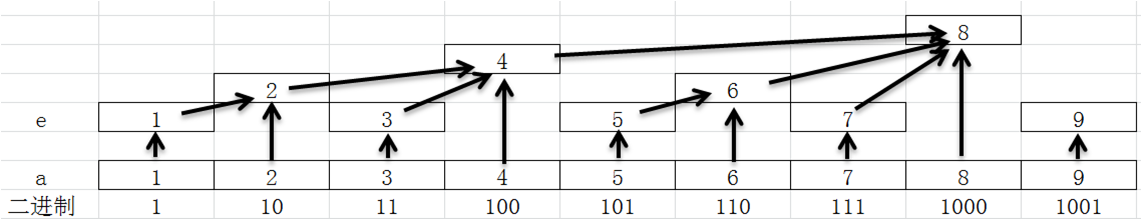
\includegraphics[width=5.0in]{img/bit.png}
    \caption{树状数组 ({\bf Fenwick Tree})}\label{fig:bit}
  \end{center}
\end{figure}
如图\ref{fig:bit},每个节点对应一个位向量,该位向量为对其子节点的位向量进行或操作后的结果。

每个节点所管辖的区间长度恰好为{\bf 节点编号的二进制表示中最低的1的位置代表的2的幂}。例如6的二进制表示为{\bf 0110},6号节点管辖的区间长度就是2。

\subsection{使用树状数组作为UpBit的组织形式}
\begin{itemize}
\item 对行查询:
  \begin{enumerate}[1.]
  \item 我们要做的是:找到最大的i,使得前i个值的位向量或操作后第k位为0。实际上val[k](第k行的值)即为i+1。
  \item 使用树状数组,我们可以从值的二进制表示中,由最高位到最低位依次确定。
  \item \begin{minted}{C++}
int get_value(int row_id) {
  int col_id = 0;
  for (int i = 0; i <= log2(n); i++) {
    if (ub[col_id+(1<<i)][row_id] ^ vb[col_id+(1<<i)][row_id] == 0) {
      col_id += (1<<i);
    }
  }
  return col_id;
}
  \end{minted}
  \end{enumerate}
\item 范围查询:
  \begin{enumerate}[1.]
  \item 树状数组求前缀和
  \item \begin{minted}{C++}
while (k > 0) {
  res |= val[k];
  k -= lowbit(k);
}
  \end{minted}
  \end{enumerate}
\end{itemize}

\section{实验结果}
\subsection{对行查询效率对比}
\begin{figure}[H]
  \begin{center}
    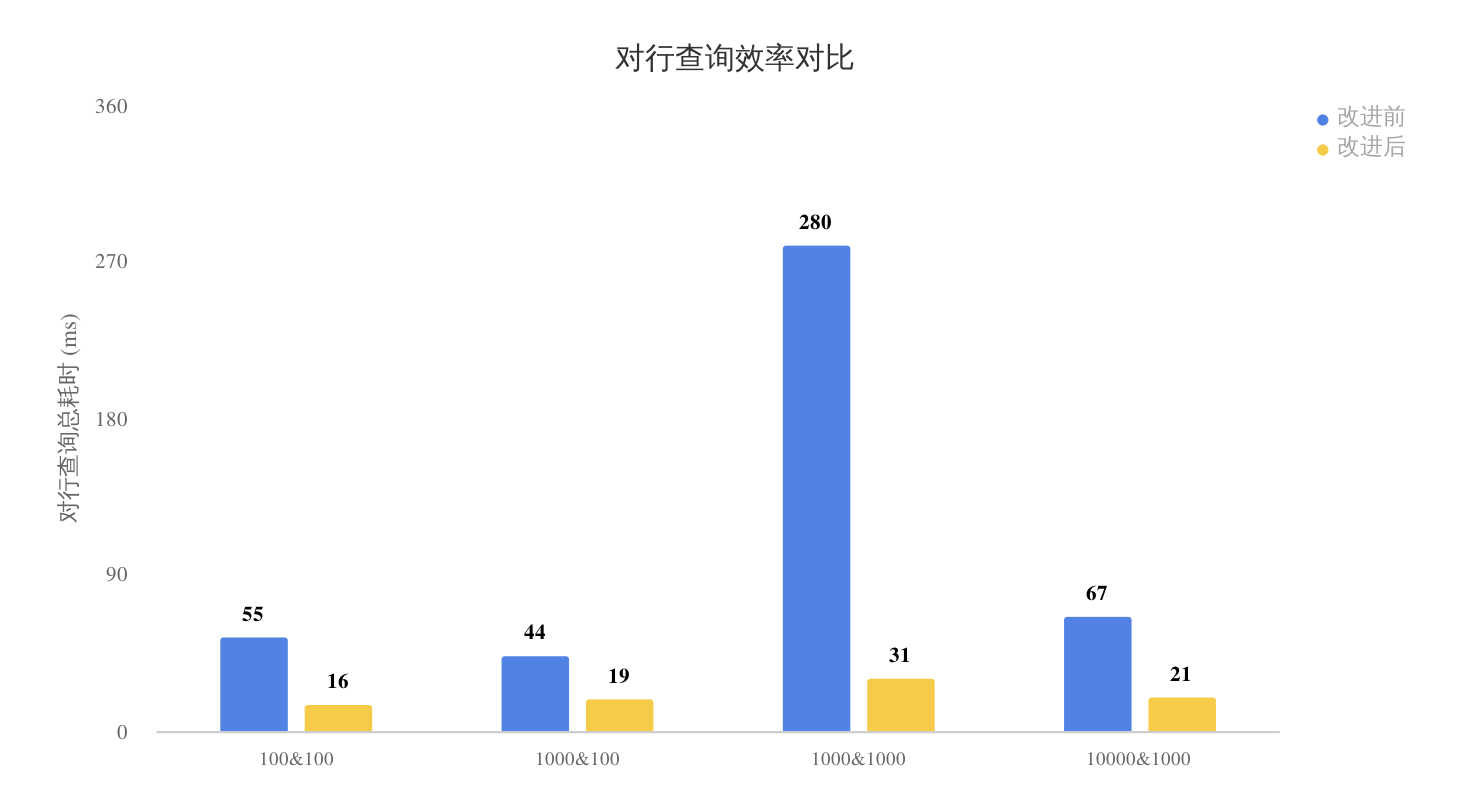
\includegraphics[width=6.5in]{img/row.png}
    \caption{对行查询效率比较图}\label{fig:row}
  \end{center}
\end{figure}
\subsection{范围查询效率对比}
\begin{figure}[H]
  \begin{center}
    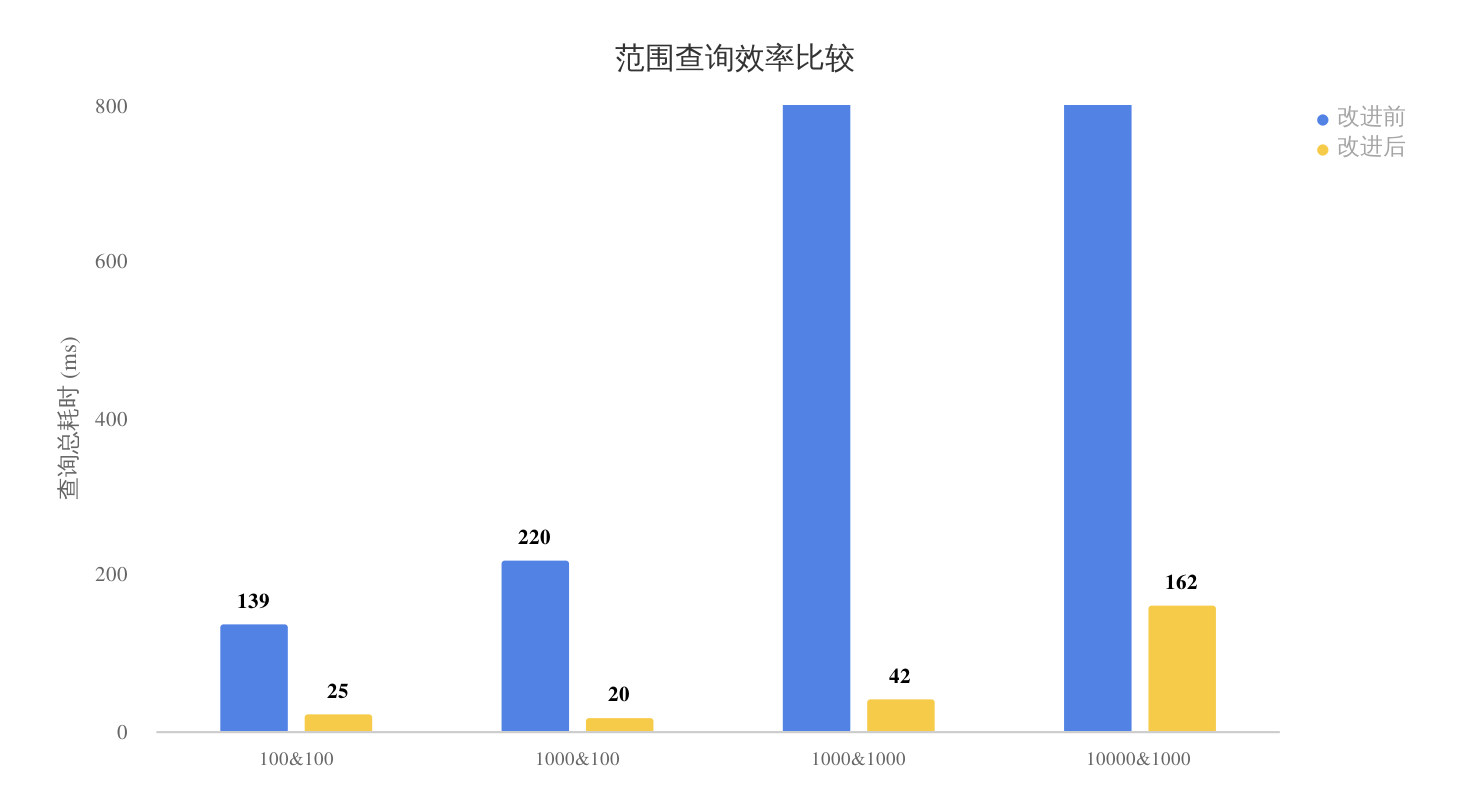
\includegraphics[width=6.5in]{img/query.png}
    \caption{范围查询效率比较图}\label{fig:query}
  \end{center}
\end{figure}
\subsection{单值修改效率对比}
\begin{figure}[H]
  \begin{center}
    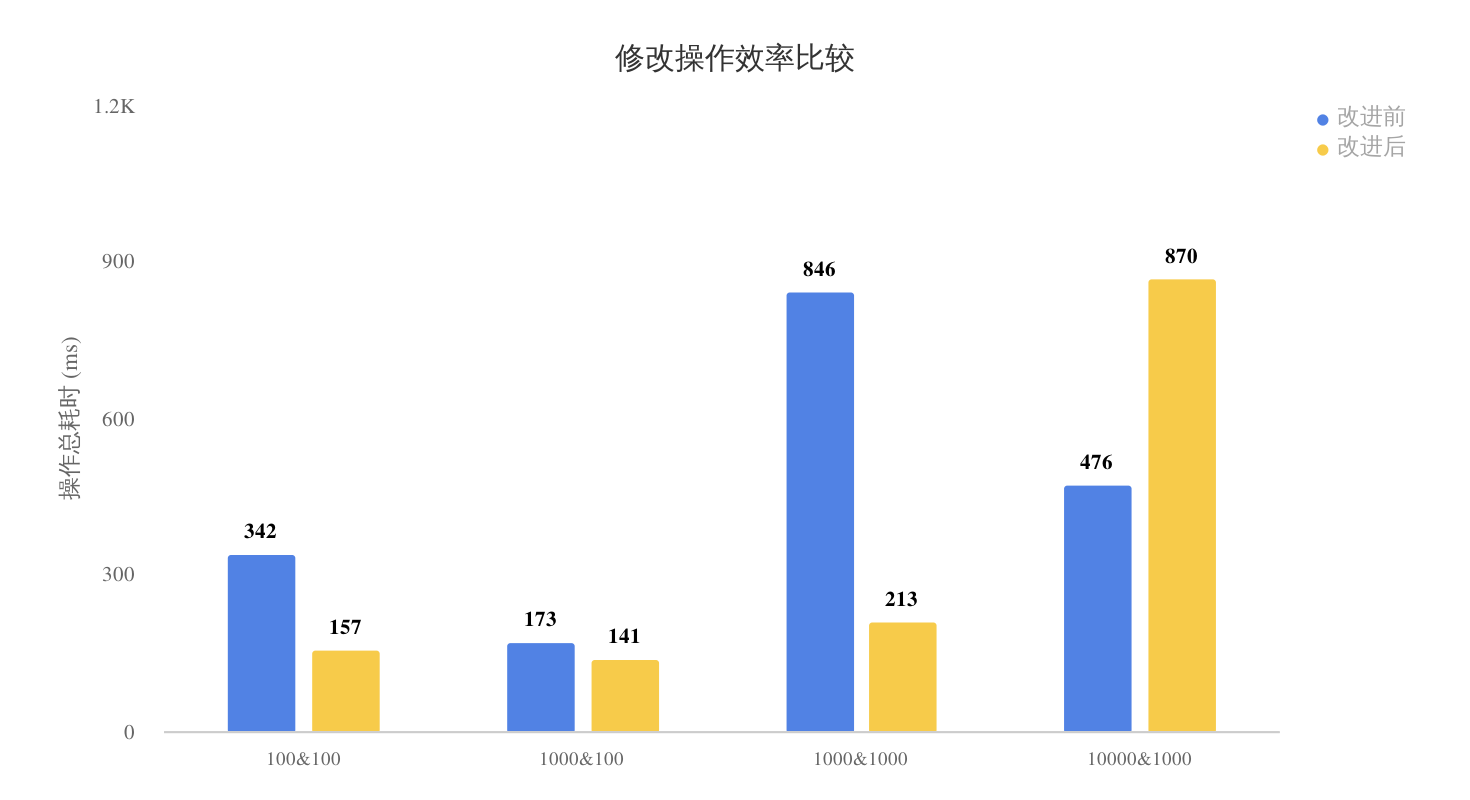
\includegraphics[width=6.5in]{img/update.png}
    \caption{修改操作效率比较图}\label{fig:update}
  \end{center}
\end{figure}

\section{结论}

\begin{itemize}
\item 改进后的UpBit对于范围查询效率更高
\item 改进后的UpBit在基数较大的情况下修改操作效率更高
\item 改进前的UpBit在基数较小的情况下修改操作效率较高
\item 如果将树状数组修改为其他平衡树(例如Splay),将能够在取值集合未知的情况下,动态向属性的取值集合添加元素。(尽管效率可能下降。)
\item 高效地利用Update BitVector将能在不影响效率的情况下减少其内存使用。
\end{itemize}


\renewcommand\refname{参考文献}
\begin{thebibliography}{99}
\bibitem{art1}Athanassoulis M, Yan Z, Idreos S. UpBit: Scalable In-Memory Updatable Bitmap Indexing[C]//Proceedings of the 2016 International Conference on Management of Data. ACM, 2016: 1319-1332.
\bibitem{art2}Canahuate G, Gibas M, Ferhatosmanoglu H. Update conscious bitmap indices[C]//Scientific and Statistical Database Management, 2007. SSBDM'07. 19th International Conference on. IEEE, 2007: 15-15.
\bibitem{art3}程鹏. 位图索引技术及其研究综述[J]. 科技信息, 2010 (26): 134-135.
\bibitem{art4}Wu K, Ahern S, Bethel E W, et al. FastBit: interactively searching massive data[C]//Journal of Physics: Conference Series. IOP Publishing, 2009, 180(1): 012053.
\bibitem{art5}Wu K, Otoo E J, Shoshani A. Compressing bitmap indexes for faster search operations[C]//Scientific and Statistical Database Management, 2002. Proceedings. 14th International Conference on. IEEE, 2002: 99-108.
\end{thebibliography}

\end{document}
